\chapter{ネットワークアクセス層 (その1)概論と二つの端点を直結するネットワーク}

今度は、インターネットプロトコル層はいったんおいておいて、インターネットプロトコルスイートを下から見ていくことにします。インターネットプロトコル層は、サービスとしてネットワークアクセス層を利用します。そのサービスについて、見ていくことにしましょう。

この章では、一番簡単なネットワークとして、二つの機器を直接繋ぐネットワークから考えていくことにします。


\section{ネットワークアクセス層}
ネットワークアクセス層というレイヤーについて説明を創める前に、もういちどその役割を定義しておこう。ネットワークアクセス層は、物理的に接続されたホストとホストの間での通信を提供するレイヤーである。インターネットプロトコルスイートにおいては、ケーブルやNICといった物理的なもの、それを利用して、接続された機器どうしの通信を提供するソフトウェアを総合したものである。

ただし、インターネットプロトコルスイートにおいて、ネットワークアクセ数層はプロトコルとしての定義があるわけではない。インターネットプロトコル層が通信のためにりっようで着るサービスであれば、なんでもかまわないということである。そのため、PPPやイーサネットという、レイヤーとしてのネットワークアクセス層に分類される規格はいずれも、インターネットプロトコルスイートで定義されたものではない。

なので、鳩でもかまわないのだ。

\subsection{同じネットワーク}
ネットワークアクセス層、そして今後説明をするインターネットプロトコル層について考えるとき、「同じネットワーク」という概念が登場する。この、同じネットワークとは何であろうか。

同じネットワーク、というのは、ネットワークアクセス層のサービスのみで通信が可能な範囲である。たとえば、本章で説明する、通信を行うエンド同士が直接接続されたネットワークは、同じネットワークということができる。同様に、次章で説明する、イーサネットによって構成されたLANに接続されたホストは、同じネットワークに接続されている、という表現になる。

また、ネットワークアクセス層の説明において、単にネットワークと表現する場合は、この「同じネットワーク」を意図している。

\subsection{違うネットワーク}

では、同じネットワークがあれば「違うネットワーク」もあるのだろうか。違うネットワークという言葉はあまり使われないが、その概念は存在する。

ネットワークアクセス層のサービスのみで通信できない、独立したネットワークが複数有るとき、それらのネットワークは互いに、。たとえば、ビルのフロア毎にLANがあるとする。そして、そのフロアとフロアの間は接続がされていない。このとき、各フロアのネットワークは、それぞれ「違うネットワークということになる。

この、違うネットワークの間での通信を行うためのレイヤーが、後の章で説明するインターネットプロトコル層である。つまり、異なるネットワークを接続するためのプロトコルであるから、「インターネット」プロトコル層、というわけだ。

これは、上位のレイヤーがかその下にあるレイヤーのサービスを利用して通信する、というこれまでの説明に照らせば、全く逆の概念のおうに思えるかもしれない。だが、ネットワークアクセス層は、インターネットプロトコル層のサービスを使用しての通信は行わないことに注意すれば、上位のレイヤーがカイノレイヤーのサービスを利用して通信する、というインターネットプロトコルスイートの原則は守られていることがわかる。

あるホストが違うネットワークに接続されたホストと通信しようとしたときに使うサービスはインターネットプロトコル層のサービスである。そのとき、ネットワークアクセス爽雨のサービスを利用するのであって、その逆ではない。

\section{いちばん簡単なネットワーク}

いちばん簡単なネットワークとは、なんであろうか。複数の機器を何らかの手段で接続したものがネットワークであるとすれば、その最小数である二つの機器を接続したものであろう。

例えば、PC2台をクロス接続のLANケーブルで接続したものがネットワークであることに、おそらく異論はないであろう。では、その2台のPCを結ぶケーブルがシリアルケーブルであっても、相互に通信をすることができればネットワークであろう。それならば、2台の機器を接続するのがパラレルケーブルでも、ネットワークになるであろう。

本章では、ネットワークアクセス層のさわりとして、二つの端点を結ぶことで校正される、最小のネットワークについての説明を行う。


\subsection{電話線を介したネットワーク}
2台のPCの間に距離があり、その接続に電話線を使用した場合は、ネットワークになるのであろうか?

そして、電話線の向こうにあるのがルータであり、電話線をネットワークアクセス層として、電話線の向こうにあるルータとインターネットプロトコルで通信できたとする。そのとき、電話線の向こうにあるルータがインターネットに接続していたらどうなるか。

ルータと電話線経由で接続すると、そのルータ経由でインターネット接続ができることにある。このとき、ルータとPCは電話線を介して直接接続されている。つまり、この電話線を用いた接続\footnote{ダイヤルアップ接続という。}は、ネットワークアクセス層である。

\subsection{一対一のネットワークに使われるインタフェイス}
二つの端点を直結するネットワークアクセス層は、電話線を介したもの以外にも存在する。たとえば、イーサネットのネットワークインタフェイスカードが高価だったり、そもそも搭載することができなかったりする場合、シリアルインタフェイスやパラレルインタフェイスを通じて、他のホストに接続する方法を取るときに使われる


\subsection{一対一のネットワークの特徴}
二つの端点を直結するネットワーク、つまり、一対一のネットワークの特徴とは何であろうか。

それは、そのネットワークにおける自分以外の存在は、必ず唯一の通信相手になるということである。これを言い換えれば、通信の相手は一つしかないのだから、自分、それ以外という以上の区別を必要としない。そのため、一対一のネットワークでは、それぞれの端点を区別する方法を持たない。

これがどういうことかというと、一対一のネットワークでは、端点にアドレスなり名前なりを付ける必要がないということである。\footnote{この概念をIP層に持ち込んだ考え方が、UnnumberdIPである。}そのため、一対一のネットワークは、実装が簡単になり、計算機のリソースも比較的小さい。

では、一対一のネットワークとして使用される規格として、SLIPとPPPを紹介することにしよう。

\section{SLIP}

シリアルケーブルを用いたネットワークアクセス層の規格に、SLIPというものがある。

SLIPとは、Serial Line IPの略で、シリアルポート接続で、IPv4のインターネットプロトコル層の通信を行うためのネットワークアクセス層プロトコルである。プロトコルの構造からIPv6にも対応可能かと思われるが、IPv6での実用例はない。

RFC1055で定義されていて、上位のインターネットプロトコルに依存した実装である。、また、SLIPには、一度で送信できるデータの長さであるフレーム長の上限がないという特徴がある。そのため、SLIPのフレーム町の最大は、次章で説明するインターネットプロトコル層から一度に送信される最大サイズのデータグラム\footnote{IPデータグラムの最大長は64kbyteとなる}となる。

SLIPのフレームは、データグラムに対して1バイトのヘッダとトレイラを追加して、フレームの最初と最後を判別できるようにしたものである。規格上はSLIPにヘッダはないが、ほとんどの実装では回線ノイズ対策としてトレイラと同じ符号を送信する。\footnote{ノイズが発生した場合、ヘッダのキャラクタがトレイラのキャラクタと同じであることを利用して、エラーの生じたデータグラムを終了させる。}

データグラム中に出現する、ヘッダと同じキャラクタを2バイトのコードでエスケープする。エスケープと同じキャラクタは、更に別の2バイトのコードでエスケープする。

ネットワークアクセス層の規格としては単純な構造である。だが、現在ではほとんど使われていない。簡単をもって尊しと為すインターネットにおいて、SLIPが使われなくなった理由として、以下が挙げられる。

\begin{itemize}
\item 両端点は予めIPアドレスが割り当ててある必要がある。IPアドレスがわからないときの問い合わせと通知という、インタフェイスとIPアドレスを動的にマッピングする機能がない。
\item エラーチェックの仕組みがない。データ破損のチェックは、IP層やトランスポート層で行う必要がある。
\item ユーザ認証に関する機能がない\footnote{ここでいうユーザ認証とは、ネットワークアクセス層での接続を許可するかの判定である}
\item インターネットプロトコル層の位置に相当するプロトコルを複数混ぜて使うことができない\footnote{イーサネットには、直上の層のプロトコルを認識するために、ヘッダにタイプフィールドがある。この機能は、TCP/IP専用ではなく、他のネットワークアクセス槽プロトコルでも使用される}
\end{itemize}

\subsection{SLIPはどこで使われていたか}

では、SLIPはどこで使われていたのだろうか。それを明らかにするには、少しばかり昔話をしなければならない。

アメリカでは、ごく初期の、ダイアルアップによるインターネット接続にSLIPが使われていた。これは、利用者に対してグローバルなIPアドレスを固定的に割り当てていたためである。\footnote{そのころはグローバルIPアドレスと言ってもアメリカしか使っていなかった。また、アメリカの大学や研究期間の関係者しかインターネットを使用する機会がなかった。}

また、現代でも、ごくまれにネットワークインタフェイスはないがシリアルインタフェイスはある、というホストに、OSのネットワークインストールを行うために使用されることもある。

SLIPは実装が簡単という利点がある。それは実装に必要なコードが少ないということであり、実行バイナリも小さいということである。そのため、フロッピーディスク起動をしなければならないOSのインストール時にも、起動メディアに導入しやすかったという事情がある。

\subsubsection{CSLIP}

TCP/IPを用いてアプリケーションが通信するとき、送信したいデータの先頭に付加する通信情報であるヘッダ部分が、データに対して大きくなりやすい。そのため、小さなデータを多量にやり取りする場合は、通信全体を通してみたときに、送信したビット列に占めるヘッダの割合が大きくなる。

それは遅い伝送媒体をネットワークアクセス層に使用する場合、より顕著な問題となる。ただでさえ遅い回線で、データの半分以上がトランスポート層とインターネットプロトコル層のヘッダで占められるという状態になってしまう。\footnote{トランスポート層でこの問題を解決する方法として、Nagleのアルゴリズムが提案されている。Nagleのアルゴリズムは、小さなデータをある程度まとめて送信することで、通信におけるヘッダの割合を減らす。}

SLIPでそれを解消する方法として、CSLIP(圧縮SLIP RFC1144)という規格が提唱された。アプリケーション間のセッションにおいて、トランスポート層のヘッダとIPヘッダの不変な部分を利用して仮想的な16 本の通信路としてセッションを管理する。そして、トランスポート層のヘッダ、IPヘッダで送出毎に変更のある部分(チェックサムなど)のみ送出することで、ヘッダを5バイト程度まで圧縮する。

\section{PPP}

次に、ダイヤルアップ接続などで名前を聞くことが多い、PPP(Point to Point Protocol)について説明しよう。

PPPは、上位層としてどのようなプロトコルを採用するかに依存しない。インターネットプロトコル以外にも、NetBIOSやAppleTalkなど、各種のプロトコルの宇手段として使用することができる。いわば、純然たるネットワークアクセス層のプロトコルである。

PPPとは、Point to Point Protocolの略で、その名の通り、一対一の通信を行うためのプロトコルである。電話線を経由したダイアルアップによるインターネットプロバイダへの接続などで、多くの場合PPPが用いられる。

\subsection{PPPの接続と切断の手順}
PPPと、先に説明したSLIPは、一対一の通信で用いられるプロトコルである。その違いは、接続手順と切断手順が存在すること、それに伴い、ネットワークアクセス層の接続について認証を行う仕組みがあることである。つまり、ネットワークアクセス層での接続の制御が可能ということだ。そのため、ダイアルアップ接続の際に、ネットワークアクセス層として用いられる。

\begin{enumerate}
\item LCP(Link Control Protocol リンク制御プロトコル)のリンク開始フレームを送信して、ネットワークアクセス層での通信条件を決定する。
\item PAP(Password Authentication Protocol パスワード認証プロトコル)やCHAP(Challenge Handshake Authentication Protocol チャレンジハンドシェークプロトコル)を使用して、接続時の認証を行うことが可能。\footnote{正確には認証情報のやり取りが可能、であり、PPPにはユーザデータベースや認証を行う機能はない。この部分はRADIUSが担当することが多い。}
\item NCP(Nwtwork Control Protocl ネットワーク制御プロトコル)のフレームを送信して、PPPを使用する上位のプロトコルの情報や、制御情報を交換する。TCP/IPであれば、必要であればエンドのIPアドレスはNCPを使って通知される。
\item 上位の層から来たデータグラムは、PPPヘッダとPPPトレイラを前後に追加されて、PPPフレームとなる。PPPヘッダにはプロトコル番号のフィールドがあり、それによって、到着先のPPPがデータグラムを渡す上位層を判別する。
\item 切断時は、LCPのリンク終了フレームを送信して、接続を終了する
\end{enumerate}

ここでわざわざ「インターネットプロトコル層」でなく「上位の層」と書いたのは、PPPは運んでいるデータグラムのプロトコルが何であるかの情報をヘッダ情報として持っているからである。そのため、AppleTalkやNetBEUIなど、TCP/IPのインターネットプロトコル層と同じ層に位置する、PPPからみた上位プロトコルも、PPPをネットワークアクセス層として使用することができる\footnote{TCP/IPほぼ一択である現在では実質的に使われることのない機能である。}

\subsection{PPPとSLIPの比較}

では、一対一の通信を実現するプロトコルであるPPPとSLIPを、表\ref{pppslip}で比較してみよう。SLIPの利点は、実装が簡単なこと、実行バイナリが小さいこと、ヘッダ情報などの通信のオーバヘッドが小さいことである。だが、ネットワークと計算機の資源が富豪化した現在では、PPPを選択することがほとんどである。\footnote{組み込みなど、計算機資源が乏しく認証の必要がない場合などは、SLIPを選択する場合があり得る。}

\begin{table}[hbtp] \caption{PPPとSLIPの比較} \label{pppslip}
\begin{center}
	\begin{tabularx}{110mm}{lXX} \toprule
		項目 & PPP & SLIP \\ \midrule
		対応する上位層プロトコル & ネットワークアクセス層の直情にくる各種プロトコル  & TCP/IPのみ \\
		エラーチェック & CRCによって行える & エラーチェックなし \\
		IPアドレス配布 & NCPで行う & 行えない。端点のIPアドレスは事前に決めておく必要がある \\
		TCP/IP通信の圧縮 & 可能 & CSLIPは可能 \\
		認証 & 可能 & 不可能 \\
		接続開始、終了 & 状態遷移がある & 状態遷移がない \\
		MTUとフラグメント & 最大1500byte 上位層でフラグメントが必要 & データグラムの上限がない \\
		実装の難易度 & 複雑 & 簡単 \\
		通信のオーバヘッド & LCPやNCPの送受信とPPPヘッダ・トレイラ & (ヘッダ)、トレイラ、エスケープ \\ \bottomrule
	\end{tabularx}
\end{center}
\end{table}

\section{ループバックインタフェイスと自分宛の通信}

\begin{figure}[htbp]
	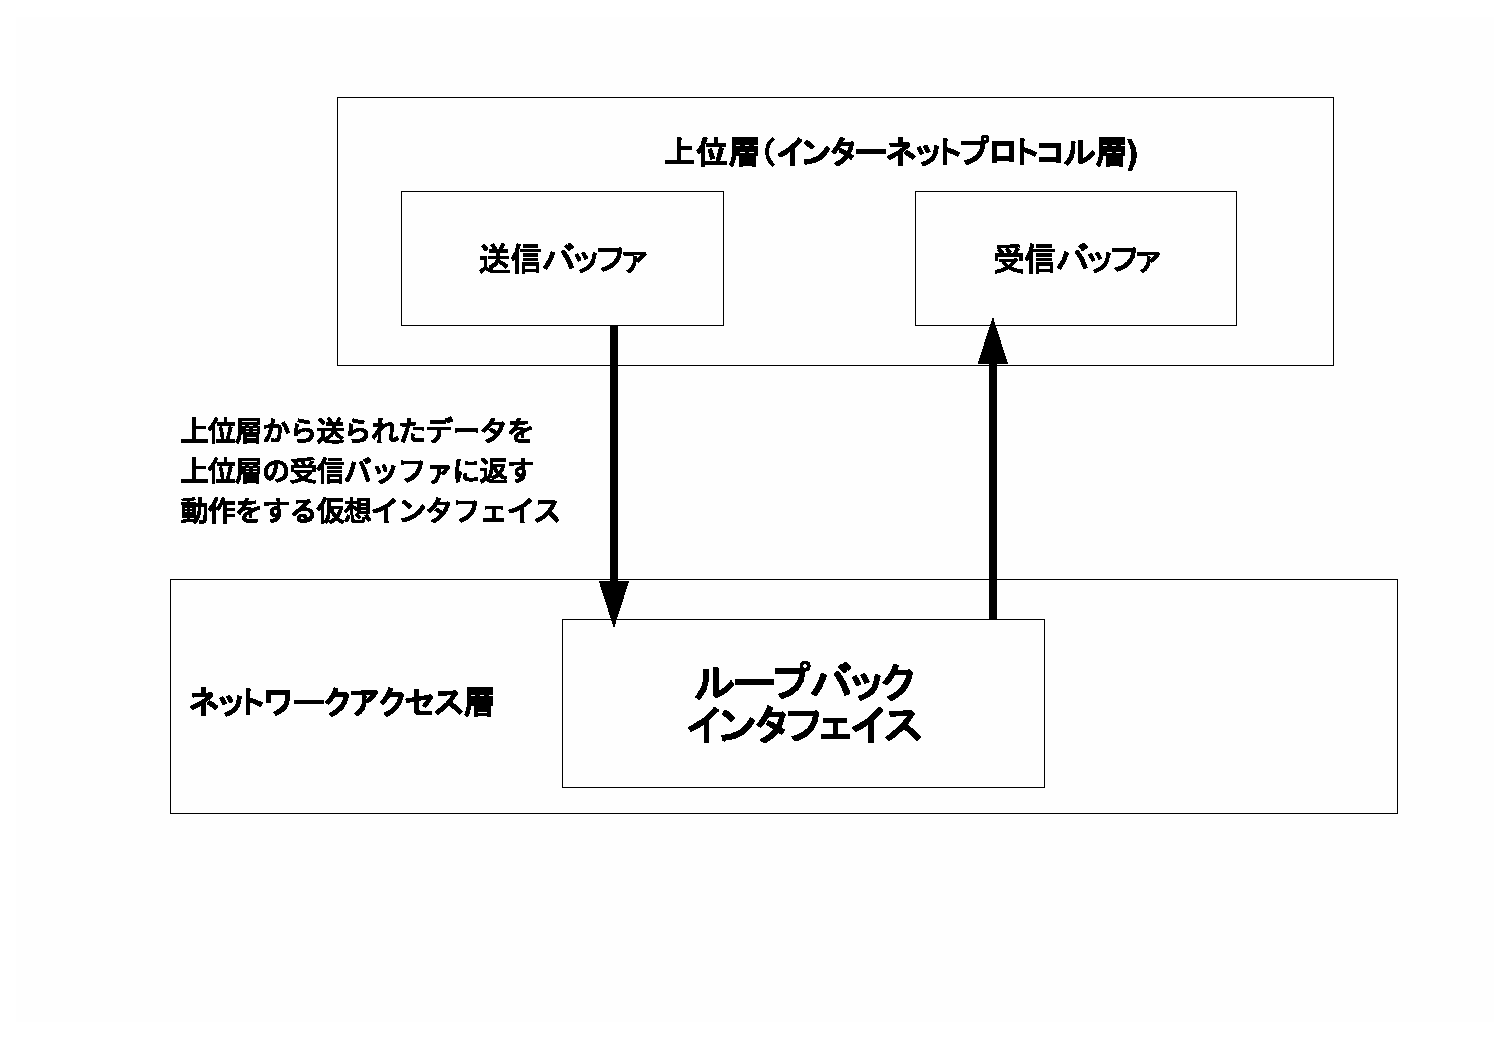
\includegraphics[width=12cm,clip]{draw/loopback.eps}
	\caption{ループバックインタフェイス}
	\label{fig:loopback}
\end{figure}

本章の最後に、仮想的な一対一通信のインタフェイスである、ループバックインタフェイスを説明しよう。では、ループバックインタフェイスは、何と何の間の通信のインタフェイスなのだろうか。

ループバックインタフェイスは、自分と自分の通信のためのインタフェイスである。

ループバックインタフェイスは、ネットワークアクセス層がインターネットプロトコル層に対して提供する、仮想的なネットワークいたフェイスである。

ループバックインタフェイスは、ループバックインタフェイス宛に送信されたデータを、そのまま自分自身のインターネットプロトコル層に、「受信したデータ」として渡す、それによって、物理的なインタフェイス、ネットワークを介さずに、自分自身とインターネットプロトコル層レベルの通信が可能となる。

つまり、同一ホスト上で動作しているアプrケーション間で、TCP/IPによるプロセス間通信が可能となるということだ。

ループバックインタフェイスは実在するインタフェイスと派対応していない。そのため、MACアドレスなど、物理デバイスと対応づけるための名前をもたない。\footnote{ifconfigコマンドでループバックインタフェイスの情報を見ると、MACアドレスは設定されていないことがわかる。}
